\section{Machine Learning}
Neural networks belong to a wider field of machine learning (ML) - the study of using experience to improve algorithms. This section assumes a basic understanding of ML and gives a brief overview of the topics needed to understand the scope of the project. It then explains in more details the background and related work for the architectures involved in this research.


\subsection{Metrics} \label{ml-accuracy-auc-confusion}
There are several key metrics used for assessing the success of an ML algorithm, and the following will be used throughout the report:

\begin{itemize}
  \item \textbf{Classification accuracy} - a simple measure of the percentage of correctly classified samples.
  \item \textbf{Area Under the Curve (AUC) for the Receiver Operator Characteristic (ROC)} - a more complex measure of the model's ability to correctly distinguish between classes. It can be used similarly to the classification accuracy, but it favors discriminative over representative models.
  \item \textbf{Confusion matrix} - a tabular metric that compares the actual samples' classes with the predicted ones, effectively categorizing results into four groups: true positive, false positive, false negative, and true negative. This allows for an easy calculation of precision and recall values.
\end{itemize}

\indo{Give equations for TPR, FPR, AUC etc.}
\indo{Explain when accuracy is not enough and AUC and confusion matrix gives a better picture}
\indo{|}


\subsection{Deep Neural Networks}
While there exist a number of ML techniques that have proven successful for various use cases at LHC, like Support Vector Machines \cite{38-valentino2012classification} or Boosted Decision Trees \cite{pmlr-v42-chen14}, in the last years deep neural networks (DNN) have been proposed with improved results for applications like infrastructure monitoring \cite{39-skoczen2016lstm}, offline data analysis \cite{40-ren2020unveiling}, and the main interest of this report - detectors' trigger mechanisms.

In many uses cases the neural networks architectures are optimized and accelerated to shorten the training time (measured in hours or even days) to reduce the time needed for evaluating different design configurations and easily performing the hyperparameter search. However, this work focuses on accelerating the inference to match the extremely low latency required in the LHC detectors' L1 triggers. Although often measured in milliseconds, sub-milliseconds inference time has been achieved for this application with the use of FPGAs using architectures for basic DNN \cite{36-kreinar2018fast}, and recently sub-microseconds latency for graph neural networks (GNN) \cite{42-kreinar2020distance-weighted, 41-elabd2021graph}. These implementations serve as a baseline latency for this project which aims to achieve comparable performance with higher AUC value.

\begin{figure}[hpt!]
  \centering
  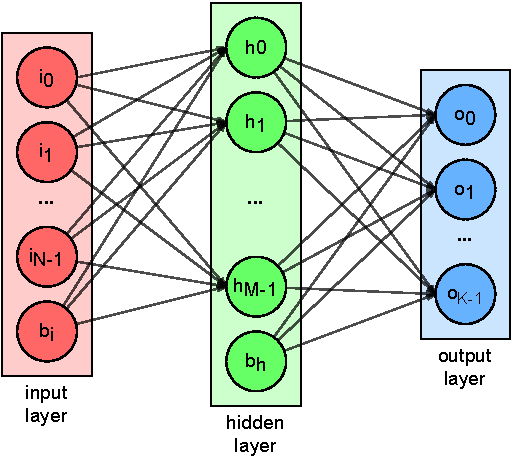
\includegraphics[trim={0cm 0cm 0cm 0cm}, width=0.4\textwidth, center]{background/fully_connected_layer.pdf}
  \caption{Diagram of a fully connected layer.}
  \label{fig:fully-connected-layer}
\end{figure}

Figure \ref{fig:fully-connected-layer} shows an overview of a fully connected neural network with one hidden layer, which allows to derive the mathematical formulae. Each layer consists of neurons which hold a value, which means that input, output and the intermediate hidden layer can be modelled similarly. The arrows between neurons represent learnable weights, while the (optional) biases involved in the calculation, denoted as \(b\), can be depicted as arrows from the "bias neurons", in all but the last layer. The value of a neuron depends on all the neurons in the previous layer as well as the weights and biases between them, which can be formulated into the equation \ref{eq:neuron} using the hidden layer as an example:

\begin{equation}\label{eq:neuron}
  h_0 = f ( w_{i, 0} \cdot i_0 + w_{i, 1} \cdot i_1 + \hdots + w_{N-1} \cdot i_{i, N-1} + b_{i, 0} )
  = f ( \sum_{j=0}^{N-1} w_{i, j} \cdot i_j + b_{i, 0} )
\end{equation}

What is also not displayed in the diagram, but can be seen in the equation is the activation function \(f\) that is required to introduce non-linearity in the computations. Without it, all consecutive layers involving solely multiplication and addition could be simplified to s a single layer thanks to the distributive property in linear algebra, defeating the point of having multiples of learnable parameters. The activation function can be as simple a piece wise linear function called Rectified Linear Unit (ReLU) defined in equation \ref{eq:relu}:

\begin{equation}\label{eq:relu}
  \text{ReLU}(x) = \text{max}(x, 0) = 
  \begin{cases}
    x & \text{x > 0} \\
    0 & \text{otherwise}
  \end{cases}
\end{equation}

or more complicated like the Sigmoid Linear Unit (SiLU), based on the sigmoid function, both presented in equation \ref{eq:silu}

\begin{equation}\label{eq:silu}
  \text{SiLU(x)} = x \cdot \sigma (x) = x \cdot \frac{1}{1 + e^{-x}}
\end{equation}

As layers are tightly connected to each other, this type of neural layer is often referred to as \textit{fully connected} or \textit{linear}. It requires a relatively large number of separate weights and biases, which makes it both computationally and memory intensive, but nonetheless, modern network architectures can have dozens of these layers, not to mention plethora of other types.


\subsection{Convolutional Neural Networks}
\indo{Quick introduction and visualization of CNNs as other notable jet-tagging algorithms use them and are mentioned in this report}
\indo{|}
\indo{|}
\indo{|}
\indo{|}
\indo{|}


\subsection{Graph and Recurrent Neural Networks}
\indo{Quick introduction and visualization of graph and recurrent (including GRU and LSTM) NNs as other notable jet-tagging algorithms use them and are mentioned in this report}
\indo{|}
\indo{|}
\indo{|}
\indo{|}
\indo{|}
\indo{|}
\indo{|}
\indo{|}
\indo{|}
\indo{|}

\subsection{Batch and Layer Normalization}
\indo{Batch norm vs layer norm as both are used in the architecture}
\indo{|}
\indo{|}
\indo{|}
\indo{|}
\indo{|}


\subsection{Transformer Neural Networks and Self-Attention}
A promising architecture that has been chosen as the topic of this project is the transformer neural network (TNN). Similarly to RNNs, TNNs were designed for sequential input data, most commonly found in natural language processing applications, however, compared to RNNs, they process all input data at once. In RNNs, convolutional \cite{72-keren2016convolutional} or attention mechanisms \cite{71-chorowski2015attention-based} are used in a recurrent manner to allow models to learn the representation and connections between different parts of the input sequence, which most commonly are words in a sentence. This limits the parallelizability as the network is handled serially - each hidden state needs to wait for the result generated by the previous one. In TNNs, a modified mechanism called self-attention \cite{44-vaswani2017attention} is used which can find global relations in a data, without relying on the temporal, sequencing information. The self-attention combines several simpler operations to achieve its strength, including linear layers, matrix multiplication and the softmax function, formula for which is presented in equation \ref{eq:softmax}.

\begin{equation}\label{eq:softmax}
  \text{softmax}(x) = \frac{exp(x_i)}{\sum exp(x_i)}
\end{equation}

Softmax can be described as mapping a vector to a ratio between each input's exponentiation result and the sum of all such values, which gives the property of the resulting vector entries sum equal to one. This characteristic means that the output can be treated as vector of probabilities, which is often exploited in the final activation layer of a neural network.

\begin{figure}[!hpt]
  \centering
  \begin{tabular}{cc}
      {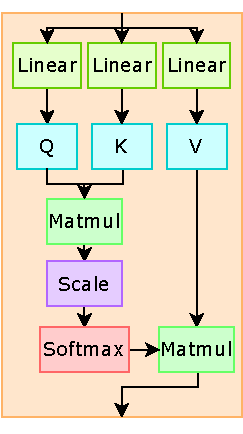
\includegraphics[width=0.2\columnwidth]{background/self_attention.pdf}} &
      {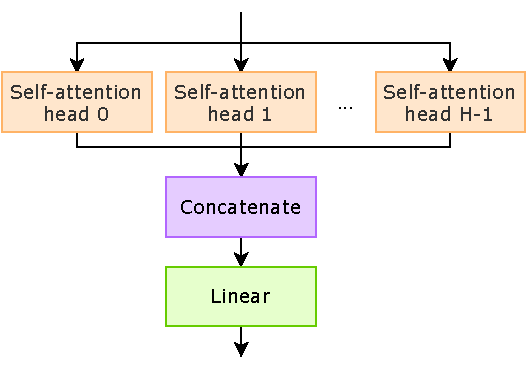
\includegraphics[width=0.4\columnwidth]{background/multi_head_self_attention.pdf}}
  \end{tabular}
  \caption{Left: diagram of a self-attention head. Right: illustration of \(H\) self-attention heads forming a multi-headed self-attention block.}
  \label{fig:self-attention-multi-head}
\end{figure}

A diagram representing the initial implementation of the self-attention can be seen on the left in figure \ref{fig:self-attention-multi-head}. The \textit{Q}, \textit{K}, and \textit{V} stand for \textit{queries}, \textit{keys}, and \textit{values} respectively, which although arbitrary, are meant to give a better understanding behind the idea of this mechanism. It is also important to note, that multiple blocks of self-attention, referred to as \textit{heads}, can be used together, which allows for each head attending information about a different hidden characteristic of an input. The results of all heads are simply concatenated, increasing output's dimensionality, and multiplied with a learned weight, as seen on the right in figure \ref{fig:self-attention-multi-head}. To better comprehend the interactions between information learned by the heads, figure \ref{fig:1-2-8-heads} shows a visualization for 1, 2 and 8 heads on an example sentence, obtained using Tensor2Tensor library \cite{tensor2tensor,73-alammarillustrated}. While it is quite clear in the example that "it" is mostly associated with "The" and "animal" with 1 attention head, the interpretability is worse in case of 2 and 8 attention heads.

\begin{figure}[!hpt]
  \centering
  \begin{tabular}{ccc}
      {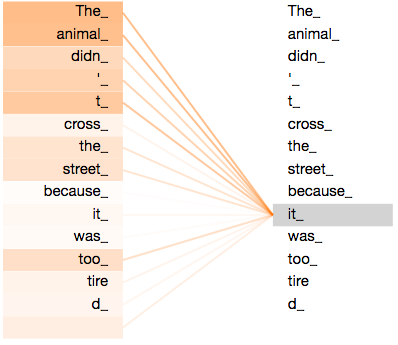
\includegraphics[width=0.32\columnwidth]{background/attention_1_head.png}} &
      {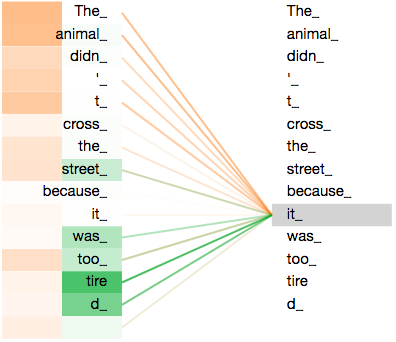
\includegraphics[width=0.32\columnwidth]{background/attention_2_head.png}} & 
      {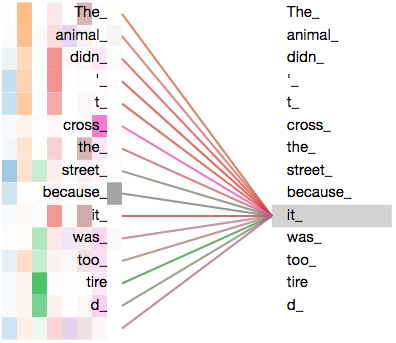
\includegraphics[width=0.32\columnwidth]{background/attention_8_head.png}}
  \end{tabular}
  \caption{From left to right: visualizations, for an input word, of the words focused by 1, 2 and 8 attention heads.}
  \label{fig:1-2-8-heads}
\end{figure}

It has to be mentioned that in terms of the AUC value, a recent implementation of a transformer called ConstituentNet \cite{3-yuan2021constituentnet:} has been shown to outperform previous state-of-the-art GNN implementations like JEDI-net \cite{9-newman2019jedi-net:} and thus serves as an inspiration for the starting point architecture of \cref{models}, which is entirely devoted to a further analysis of the network design and suitability for jet tagging. More specifically, given the strong results of its software implementation, an FPGA-mapped design is believed to have a possibility to be a viable alternative to existing designs for L1T at LHC.